%%%%%%%%%%%%%%%%%%%%%%%%%%%%%%%%%%%%%%%%%%%%%%%%%%%%%%%%%%%%%%%%%%%%%%%%%%%%%%%%
\exercice{Stabilité d'un système du second ordre}
%%%%%%%%%%%%%%%%%%%%%%%%%%%%%%%%%%%%%%%%%%%%%%%%%%%%%%%%%%%%%%%%%%%%%%%%%%%%%%%%
%%%%%%%%%%%%%%%%%%%%%%%%%%%%%%%%%%%%%%%%%%%%%%%%%%%%%%%%%%%%%%%%%%%%%%%%%%%%%%%%
\question{\textbf{À partir du critère de Routh, déterminer les conditions 
sur $K$, $\xi$ et $\omega_0$ pour deux types de fonctions de transferts $C(p)$:}
}
%%%%%%%%%%%%%%%%%%%%%%%%%%%%%%%%%%%%%%%%%%%%%%%%%%%%%%%%%%%%%%%%%%%%%%%%%%%%%%%%
%%%%%%%%%%%%%%%%%%%%%%%%%%%%%%%%%%%%%%%%%%%%%%%%%%%%%%%%%%%%%%%%%%%%%%%%%%%%%%%%
\paragraph{$C(p)=1$ (gain pur)}
%%%%%%%%%%%%%%%%%%%%%%%%%%%%%%%%%%%%%%%%%%%%%%%%%%%%%%%%%%%%%%%%%%%%%%%%%%%%%%%%
Dans ce cas la fonction de transfert en boucle fermée s'écrit :
\[
H_{BF}=
\dfrac{H(p)}{1+H(p)}=
\dfrac{K\omega_0^2}{p^2+2\xi\omega_0p+\omega_0^2(1+K)}
\]
Cette fonction de transfert est du deuxième ordre.
Le critère de Routh s'applique sur le dénominateur $D(p)$ de la fonction de 
transfert en boucle fermée.
\[
D(p)=p^2+2\xi\omega_0p+\omega_0^2(1+K)
\]
\`A l'aide du premier critère de Routh (condition nécessaire de stabilité), nous
savons que tous les coéfficients du polynôme $D(p)$ doivent être de même signe.
Il s'avère que cette condition est suffisante dans le cas où le système est 
d'ordre $n<2$.
%-------------------------------------------------------------------------------
\begin{align*}
    1+K>0 &\Rightarrow K > -1\\
    2\xi\omega_0 > 0 &\Rightarrow \xi> 0
\end{align*}
%-------------------------------------------------------------------------------
Nous retrouvons un résultat déjà connu pour la stabilité d'un système du 
second ordre amorti. En effet, le cas $\xi=0$ correspond au cas de l'oscillateur
harmonique instable par définition. Les deux autres régimes connus s'obtiennent 
pour $\xi>0$.
%%%%%%%%%%%%%%%%%%%%%%%%%%%%%%%%%%%%%%%%%%%%%%%%%%%%%%%%%%%%%%%%%%%%%%%%%%%%%%%%
\paragraph{$C(p)=\dfrac{1}{p}$ (un intégrateur)}
%%%%%%%%%%%%%%%%%%%%%%%%%%%%%%%%%%%%%%%%%%%%%%%%%%%%%%%%%%%%%%%%%%%%%%%%%%%%%%%%
Dans ce cas la fonction de transfert en boucle fermée s'écrit :
\[
H_{BF}=\dfrac{C(p)H(p)}{1+C(p)H(p)}=
       \dfrac{K\omega_0^2}{p(p^2+2\xi\omega_0p+\omega_0^2)+K\omega_0^2}
\]
Cette fonction de transfert est du troisième ordre.
Le critère de Routh s'applique sur le dénominateur $D(p)$ de la fonction 
de transfert en boucle fermée.
\[
D(p)=p^3+2\xi\omega_0p^2+\omega_0^2p+K\omega_0^2
\]
\`A l'aide du premier critère de Routh (condition nécessaire de stabilité), nous
savons que tous les coéfficients du polynôme $D(p)$ doivent être de même signe.
Soit alors les conditions suivantes, nécessaire mais pas suffisante, sur les 
paramètres du système du second ordre :
%-------------------------------------------------------------------------------
\begin{align*}
    \omega_0^2&>0 \\
    K&>0 \\
     2\omega_0\xi > 0 \Rightarrow\xi&> 0\:\:\text{( que si $\omega_0>0$)}
\end{align*}
%-------------------------------------------------------------------------------
Notons que la condition sur $K$ est différente par rapport au cas du second 
ordre pur et que la condition sur $\xi$ est retrouvée que si on impose 
une condition sur $\omega_0$ (condition physique d'une pulsation positive). 
Construisons le tableau de Routh pour permettre de déterminer les conditions 
supplémentaires.
\[
\begin{matrix}
    p^3 \\
    p^2 \\
    \hline
    p^1 \\
    p^0 \\
\end{matrix}
\begin{vmatrix}
    1     & \omega_0^2  \\
    2\xi\omega_0    & K\omega_0^2  \\
    \hline
    A_{31}\DoTikzmark{-1.2ex}{7ex}{n1}  & 0  \\
    A_{41}\DoTikzmark{-1.2ex}{0ex}{n2}  & 0    
    \end{vmatrix}
\]
\colrow[blue,opacity=.2]{n1}{n2}
avec
\[
A_{31}=-\dfrac{1}{2\xi\omega_0}
        \begin{vmatrix}
        1&\omega_0^2\\
        2\xi\omega_0&K\omega_0^2
        \end{vmatrix}
      = \dfrac{1}{2\xi\omega_0}(2\xi\omega_0^3-K\omega_0^2) = 
      \dfrac{1}{2\xi\omega_0}\left(\omega_0^2(2\xi\omega_0-K)\right)
\]
et
\[
A_{41}=-\dfrac{1}{A_{31}}
       \begin{vmatrix}
       2\xi\omega_0 & K\omega_0^2 \\
       A_{31} & 0
       \end{vmatrix}
      =K\omega_0^2
\]
Les conditions sur la colonne des pivots du tableau de Routh sont :
%-------------------------------------------------------------------------------
\begin{align*}
    2\xi\omega_0 &> 0 \\
    A_{31} &> 0 \Rightarrow \dfrac{1}{2\xi\omega_0}
    \left(\omega_0^2(2\xi\omega_0-K)\right) > 0 \Rightarrow 2\xi\omega_0-K > 0 
    \Rightarrow K < 2\xi\omega_0\\
    K\omega_0^2 &> 0 
\end{align*}
%-------------------------------------------------------------------------------
La première et la dernière conditions étaient déjà connues à partir de la 
condition nécessaire. La condition fondamentale de stabilité reliant tout 
les paramères du système du second ordre 
en série avec un intégrateur pur est :
\[
K < 2\xi\omega_0
\]
%%%%%%%%%%%%%%%%%%%%%%%%%%%%%%%%%%%%%%%%%%%%%%%%%%%%%%%%%%%%%%%%%%%%%%%%%%%%%%%%
%%%%%%%%%%%%%%%%%%%%%%%%%%%%%%%%%%%%%%%%%%%%%%%%%%%%%%%%%%%%%%%%%%%%%%%%%%%%%%%%
\exercice{Application du critère de Routh}
%%%%%%%%%%%%%%%%%%%%%%%%%%%%%%%%%%%%%%%%%%%%%%%%%%%%%%%%%%%%%%%%%%%%%%%%%%%%%%%%
%%%%%%%%%%%%%%%%%%%%%%%%%%%%%%%%%%%%%%%%%%%%%%%%%%%%%%%%%%%%%%%%%%%%%%%%%%%%%%%%
%%%%%%%%%%%%%%%%%%%%%%%%%%%%%%%%%%%%%%%%%%%%%%%%%%%%%%%%%%%%%%%%%%%%%%%%%%%%%%%%
\question{\textbf{Déterminer la stabilité des systèmes définits par les 
équations caractéristiques suivantes :}}
%%%%%%%%%%%%%%%%%%%%%%%%%%%%%%%%%%%%%%%%%%%%%%%%%%%%%%%%%%%%%%%%%%%%%%%%%%%%%%%%
\noindent~\textbf{a)}\\
La condition nécessaire du critère de Routh est trivialement respectée.
Construisons le tableau de Routh :
\[
\begin{matrix}
    p^5 \\[1em]
    p^4 \\[1em]
    \hline
    p^3 \\[1em]
    p^2 \\[1em]
    p^1 \\[1em]
    p^0 
\end{matrix}
\begin{vmatrix}
    1\DoTikzmark{0ex}{2ex}{n1}      & 3   & 3 \\[1em]
    2      & 4   & 1 \\[1em]
    \hline
    1\DoTikzmark{0ex}{-16ex}{n2}   & \frac{5}{2} & 0 \\[1em]
    -1                            & 1  & 0 \\[1em]
    \frac{7}{2}  & 0  &  0 \\[1em]
    1            & 0  &  0 
\end{vmatrix}
\]
\colrow[blue,opacity=.2]{n1}{n2}[18pt]
Avec, 
\[
A_{31}=-\dfrac{1}{2}\begin{vmatrix}1 & 3 \\2&4\end{vmatrix}=1,
\]
\[
A_{32}=-\dfrac{1}{2}\begin{vmatrix}1 & 3 \\2&1\end{vmatrix}=\dfrac{5}{2},
\]
\[
A_{41}=-\begin{vmatrix}2 & 4 \\1&\frac{5}{2}\end{vmatrix}=-1,
\]
\[
A_{42}=-\begin{vmatrix}2 & 1 \\1&0\end{vmatrix}=1,
\]
\[
A_{51}=-\begin{vmatrix}1&\frac{5}{2}\\-1&1\end{vmatrix}=\dfrac{7}{2},
\]
\[
A_{61}=-\dfrac{2}{7}\begin{vmatrix}1 & -1 \\\frac{7}{2}&0\end{vmatrix}=1,
\]
Le système est \textbf{instable} en boucle fermée par le critère de Routh.
\noindent~\textbf{b)}\\
La condition nécessaire du critère de Routh est trivialement respectée.
Construisons le tableau de Routh :
\[
\begin{matrix}
    p^4 \\[1em]
    p^3 \\[1em]
    \hline
    p^2 \\[1em]
    p^1 \\[1em]
    p^0 
\end{matrix}
\begin{vmatrix}
    1      & 3   & 1 \\[1em]
    1      & 1   & 0 \\[1em]
    \hline
    2\DoTikzmark{0ex}{12ex}{n1}   & 1 & 0 \\[1em]
    \frac{1}{2}    & 0  & 0 \\[1em]
    1\DoTikzmark{0ex}{-2ex}{n2}  & 0  &  0 
\end{vmatrix}
\]
\colrow[blue,opacity=.2]{n1}{n2}[18pt]
Avec, 
\[
A_{31}=-\begin{vmatrix}1 & 3 \\1&1\end{vmatrix}=2,
\]
\[
A_{32}=-\begin{vmatrix}1 & 1 \\1&0\end{vmatrix}=1,
\]
\[
A_{41}=-\dfrac{1}{2}\begin{vmatrix}1 & 1 \\2&1\end{vmatrix}=\dfrac{1}{2},
\]
\[
A_{51}=-\dfrac{1}{A_{41}}\begin{vmatrix}2 & 1 \\A_{41}&0\end{vmatrix}=1,
\]
Le système est \textbf{stable} en boucle fermée par le critère de Routh.
\noindent~\textbf{c)}\\
La condition nécessaire du critère de Routh est trivialement respectée.
Construisons le tableau de Routh :
\[
\begin{matrix}
    p^5 \\[1em]
    p^4 \\[1em]
    \hline
    p^3 \\[1em]
    p^2 \\[1em]
    p^1 \\[1em]
    p^0 
\end{matrix}
\begin{vmatrix}
    1\DoTikzmark{-0.5ex}{2ex}{n1}      & 3   & 5 \\[1em]
    2\DoTikzmark{-0.5ex}{-22ex}{n2}      & 6   & 3 \\[1em]
    \hline
    \epsilon   & \frac{7}{2} & 0 \\[1em]
    6-\frac{7}{\epsilon}    & 3  & 0 \\[1em]
    A_{51} & 0  &  0 \\[1em]
    3            & 0  &  0 
\end{vmatrix}
\]
\colrow[blue,opacity=.2]{n1}{n2}[30pt]
Avec
\[
A_{31}=-\dfrac{1}{2}\begin{vmatrix}1 & 3 \\2&6\end{vmatrix}=0,
\]
lorque l'on obtient un zéro dans la première colonne on remplace le zéro 
par un epsilon que l'on fait tendre vers zéro (c.a.d $\epsilon\rightarrow0$).
\[
A_{32}=-\dfrac{1}{2}\begin{vmatrix}1 & 5 \\2&3\end{vmatrix}=\dfrac{7}{2},
\]
\[
A_{41}=-\dfrac{1}{\epsilon}
       \begin{vmatrix}
           2 & 6 \\
           \epsilon&\frac{7}{2}
       \end{vmatrix}
      =6-\frac{7}{\epsilon},
\]
\[
A_{42}=-\dfrac{1}{\epsilon}\begin{vmatrix}2 & 3 \\\epsilon&0\end{vmatrix}=3,
\]
\[
A_{51}=-\dfrac{1}{A_{41}}
       \begin{vmatrix}
       \epsilon & \frac{7}{2} \\
        A_{41}&3
       \end{vmatrix}
      =\dfrac{7}{2}-3\epsilon\dfrac{1}{A_{41}},
\]
Déterminons les signes des éléments de la colonne des pivots
du tableau de Routh :
%-------------------------------------------------------------------------------
\begin{align*}
\epsilon >0 \Rightarrow \epsilon\rightarrow0^+ \\
    A_{41}=\lim\limits_{\epsilon\rightarrow 0^+}6-\frac{7}{\epsilon} <0  \\
    A_{51}=\lim\limits_{\epsilon\rightarrow 0^+}
    \dfrac{7}{2}-3\epsilon\dfrac{1}{A_{41}} >0 \\
    A_{61}=3 > 0
\end{align*}
%-------------------------------------------------------------------------------
Le système est \textbf{instable} en boucle fermée par le critère de Routh.
Le nombre de changement de signe dans la colonne des pivots nous indique le 
nombre de pôles à partie réelle positive.
\noindent~\textbf{d)}\\
La condition nécessaire du critère de Routh est trivialement respectée.
Construisons le tableau de Routh :
\[
\begin{matrix}
    p^5 \\[1em]
    p^4 \\[1em]
    \hline
    p^3 \\[1em]
    p^2 \\[1em]
    p^1 \\[1em]
    p^0 
\end{matrix}
\begin{vmatrix}
    1  & 6   & 8 \\[1em]
    7  & 42  & 56 \\[1em] 
    \hline
    A_{31} & A_{32} & 0\\[1em]
    A_{41} & A_{42} & 0\\[1em]
    A_{51} & 0      & 0\\[1em]
    A_{61} & 0 & 0
\end{vmatrix}
\]
Notons qu'il est possible de factoriser une ligne par un entier :
\[
\begin{matrix}
    p^5 \\[1em]
    p^4 \\[1em]
    \hline
    p^3 \\[1em]
    p^2 \\[1em]
    p^1 \\[1em]
    p^0 
\end{matrix}
\begin{vmatrix}
    1  & 6   & 8 \\[1em]
    1  & 6   & 8 \\[1em] 
    \hline
    A_{31} & A_{32} & 0\\[1em]
    A_{41} & A_{42} & 0\\[1em]
    A_{51} & 0      & 0\\[1em]
    A_{61} & 0 & 0
\end{vmatrix}
\]
Avec,
\[
A_{31}=-\dfrac{1}{7}\begin{vmatrix}1 & 6 \\ 1& 6\end{vmatrix} = 0
\]
et 
\[
A_{32}=-\dfrac{1}{7}\begin{vmatrix}1 & 8 \\ 1& 8\end{vmatrix} = 0
\]
Lorsque l'on a à faire à une ligne de zéro on peut remplacer cette ligne 
par la dérivée de l'équation auxiliaire. Cette équation correspond au polynôme 
construit à partir des coefficients précédent la ligne de zéros.
L'équation auxiliaire $A(p)$ est donc :
\[
A(p)=p^4+6p^2+8
\]
sa dérivée :
\[
4p^3+12p
\]
Le tableau de Routh devient alors :
\[
\begin{matrix}
    p^5 \\[1em]
    p^4 \\[1em]
    \hline
    p^3 \\[1em]
    p^2 \\[1em]
    p^1 \\[1em]
    p^0 
\end{matrix}
\begin{vmatrix}
    1  & 6   & 8 \\[1em]
    1  & 6   & 8 \\[1em] 
    \hline
    4 & 12 & 0\\[1em]
    A_{41} & A_{42} & 0\\[1em]
    A_{51} & 0      & 0\\[1em]
    A_{61} & 0 & 0
\end{vmatrix}
\]
avec 
\[
A_{41}=-\dfrac{1}{4}\begin{vmatrix}1 & 6 \\ 4& 12\end{vmatrix}=3, 
\]
\[
A_{42}=-\dfrac{1}{4}\begin{vmatrix}1 & 8 \\ 4& 0\end{vmatrix}=8,
\]
\[
\begin{matrix}
    p^5 \\[1em]
    p^4 \\[1em]
    \hline
    p^3 \\[1em]
    p^2 \\[1em]
    p^1 \\[1em]
    p^0 
\end{matrix}
\begin{vmatrix}
    1  & 6   & 8 \\[1em]
    1  & 6   & 8 \\[1em] 
    \hline
    4 & 12 & 0\\[1em]
    3 & 8 & 0\\[1em]
    A_{51} & 0      & 0\\[1em]
    A_{61} & 0 & 0
\end{vmatrix}
\]
Calculons maintenant :
\[
A_{51}=-\dfrac{1}{3}\begin{vmatrix}4 & 12 \\ 3& 8\end{vmatrix}=\dfrac{4}{3},
\]
et
\[
A_{61}=-\dfrac{1}{A_{51}}\begin{vmatrix}3 & 8 \\ A_{51}& 0\end{vmatrix}=8
\]
\[
\begin{matrix}
    p^5 \\[1em]
    p^4 \\[1em]
    \hline
    p^3 \\[1em]
    p^2 \\[1em]
    p^1 \\[1em]
    p^0 
\end{matrix}
\begin{vmatrix}
    1\DoTikzmark{0ex}{2ex}{n1}    & 6 & 8 \\[1em]
    1\DoTikzmark{0ex}{-20ex}{n2}  & 6 & 8 \\[1em] 
    \hline
    4 & 12 & 0\\[1em]
    3 & 8 & 0\\[1em]
    \frac{4}{3} & 0      & 0\\[1em]
    8 & 0 & 0
\end{vmatrix}
\]
\colrow[blue,opacity=.2]{n1}{n2}[18pt]
Le système est \textbf{stable} en boucle fermée par le critère de Routh.
%%%%%%%%%%%%%%%%%%%%%%%%%%%%%%%%%%%%%%%%%%%%%%%%%%%%%%%%%%%%%%%%%%%%%%%%%%%%%%%%
%%%%%%%%%%%%%%%%%%%%%%%%%%%%%%%%%%%%%%%%%%%%%%%%%%%%%%%%%%%%%%%%%%%%%%%%%%%%%%%%
\exercice{Critère de Nyquist~\difficile}
%%%%%%%%%%%%%%%%%%%%%%%%%%%%%%%%%%%%%%%%%%%%%%%%%%%%%%%%%%%%%%%%%%%%%%%%%%%%%%%%
%%%%%%%%%%%%%%%%%%%%%%%%%%%%%%%%%%%%%%%%%%%%%%%%%%%%%%%%%%%%%%%%%%%%%%%%%%%%%%%%
La FTBO présentant 2 pôles instables ($P=2$), le système sera stable 
en boucle fermée pour $N=2$, il existe une seule région du lieu de Nyquist de 
la FTBO pouvant prétendre à celà. La figure ci-dessous présente les différentes
valeurs de $N$ pour l'ensemble du plan complexe.  
%-------------------------------------------------------------------------------
\begin{figure}[!h]
    \centering
    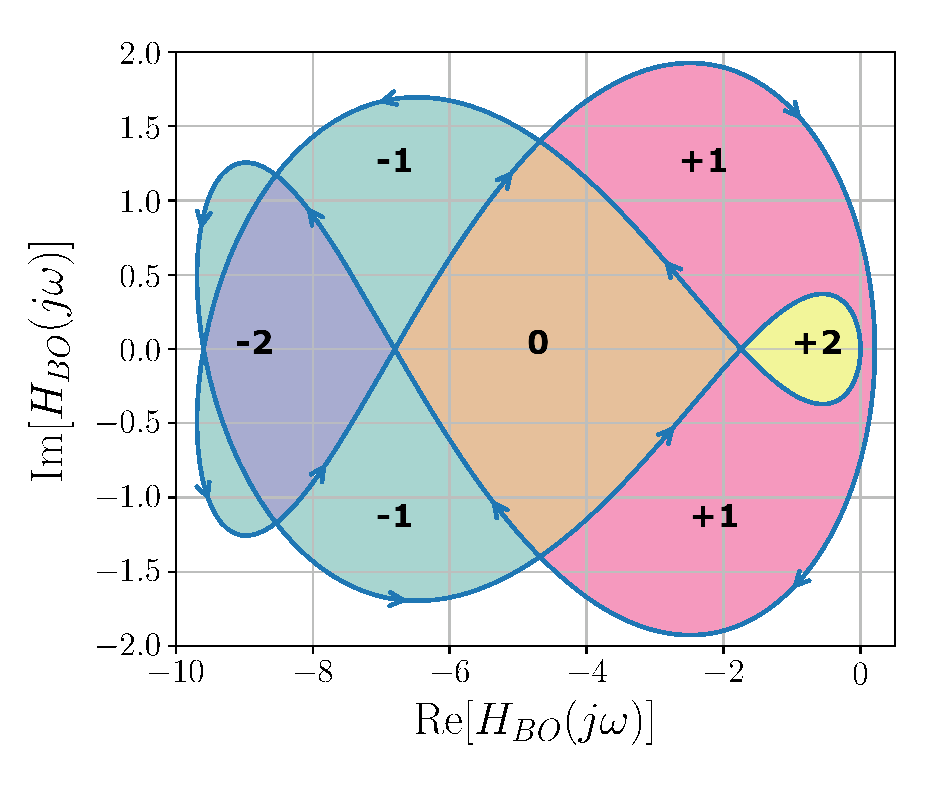
\includegraphics[width=0.8\textwidth]
                    {exercice_nyquist_chap_stab_ex3_corrige_N.eps}
\end{figure}
%-------------------------------------------------------------------------------
%%%%%%%%%%%%%%%%%%%%%%%%%%%%%%%%%%%%%%%%%%%%%%%%%%%%%%%%%%%%%%%%%%%%%%%%%%%%%%%%
\question{\textbf{Déterminer alors la condition sur $K$ pour ce système 
soit stable en boucle fermée.}}
%%%%%%%%%%%%%%%%%%%%%%%%%%%%%%%%%%%%%%%%%%%%%%%%%%%%%%%%%%%%%%%%%%%%%%%%%%%%%%%%
Pour que le système soit stable en boucle fermée, il faut que le point 
critique de coordonnées (-1,0) se trouve entre les deux points I$_1$ et 
I$_2$ comme représentés sur la figure ci-dessous.
La partie réel de ces points est directement proportionnelle au 
gain de la boucle ouverte. Lorsque l'on augmente ou diminue le gain $K$, 
le diagramme de Nyquist est tranformé par homothétie (même forme et 
même orientation).
%-------------------------------------------------------------------------------
\begin{figure}[!h]
    \centering
    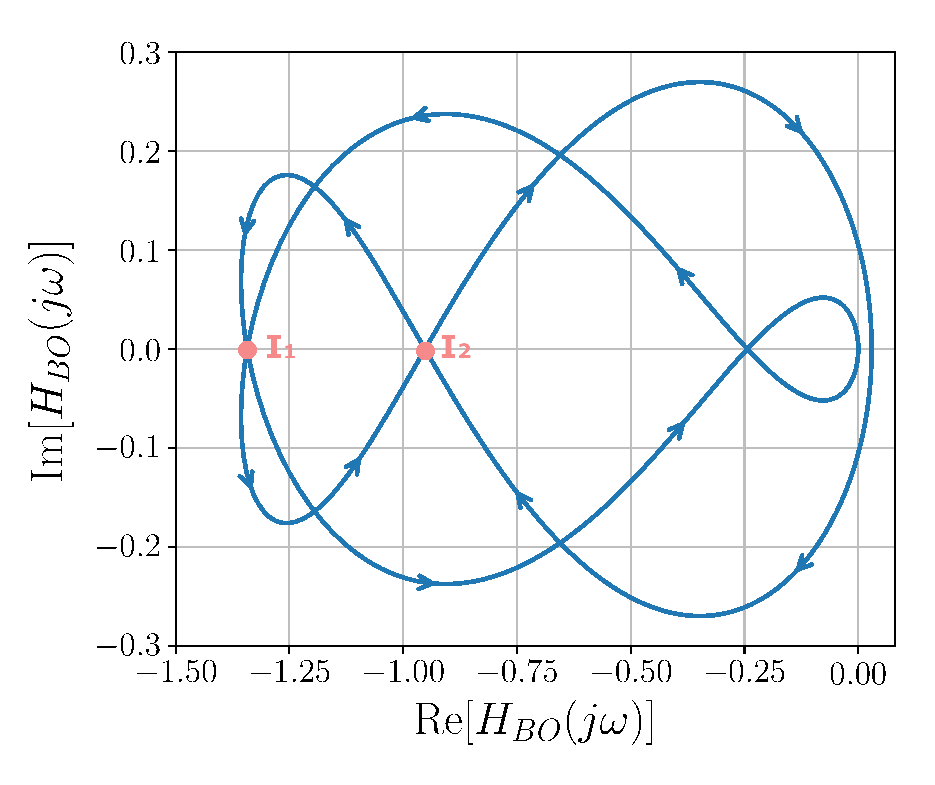
\includegraphics[width=0.8\textwidth]
                    {exercice_nyquist_chap_stab_ex3_corrige_stable.eps}
\end{figure}
%-------------------------------------------------------------------------------
Ainsi, la relation entre $K$ et cet interval est donnée par :
\[
\begin{cases}
    K\Re{\mathrm{I}_1} < 1 \\
    K\Re{\mathrm{I}_2} > 1 
\end{cases}\quad\textrm{}
\]
ou encore :
%-------------------------------------------------------------------------------
\begin{align*}
    \dfrac{1}{\Re{\mathrm{I}_1}}<K<\dfrac{1}{\Re{\mathrm{I}_2}} \\
\end{align*}
%-------------------------------------------------------------------------------
On mesure sur le diagramme précédent la position des points I$_1$ et I$_2$ 
dans le cas où $K=1$.
%-------------------------------------------------------------------------------
\begin{align*}
    \Re{\mathrm{I}_1}&=-9.59\\
    \Re{\mathrm{I}_2}&=-6.8\\
\end{align*}
%-------------------------------------------------------------------------------
donc, le système est stable en boucle fermée pour un gain $K$ tel que
%-------------------------------------------------------------------------------
\begin{align*}
    0.104&<K<0.147.
\end{align*}
%-------------------------------------------------------------------------------
Nous laissons au lecteur la vérification de cette conclusion par d'autres 
approches (critères algébriques ou graphiques).
À noter que la figure précédente a été obtenu pour un gain de $K=0.14$, plaçant
effectivement le point critique entre les points I$_1$ et I$_2$.
